\section{Methodology of BERT}

BERT is a powerful natural language processing (NLP) model developed by Google in 2018. It based on the bidirectional architecture to understand context of words by consider the words before and after them in the sentence. It can be configured to handle multiple type of tasks, the classification task like this sentiment identifying is one of its ability. Hugging Face is an open-source platform and popular for its "Transformers" library, which provides utilities to work with models like BERT. This platform do not maintain the model, but it plays a key role in BERT used widely. Hugging Face hosts pre-trained BERT models and provides code for model using, and established a community for fine tuning and deploying models for verity tasks. BERT and Hugging Face empower developers to tackle a wide range of NLP tasks efficiently.

BERT comes in several variants, each designed for different needs:

\begin{itemize}
    \item BERT-Base: A smaller model with 12 layers, suitable for tasks with limited computational resources like this task.
    \item BERT-Large: A larger model with 24 layers, offering higher accuracy but requiring more computing resource such as GPUs and memory.
    \item DistilBERT: A distilled and lighter version model with fewer parameters, faster and less resource requirements but slightly less accurate.
    \item Multilingual BERT: Trained on textual content from multiple languages, it is useful for non-English or cross-lingual tasks.
\end{itemize}

BERT is the resource and time consuming method due to it based on transformer architecture and attention mechanism. We selected the "BERT-Base" model for this task, it balanced the resources consuming and accuracy of the results. The powerful environment should be used to drive this experiment. We selected the Kaggle platform to handle this task by configuring the system using P100 GPU. It includes CUDA cores and up to 16Gb memory, which support this implementation well.

\begin{figure}[ht]
    \centering
    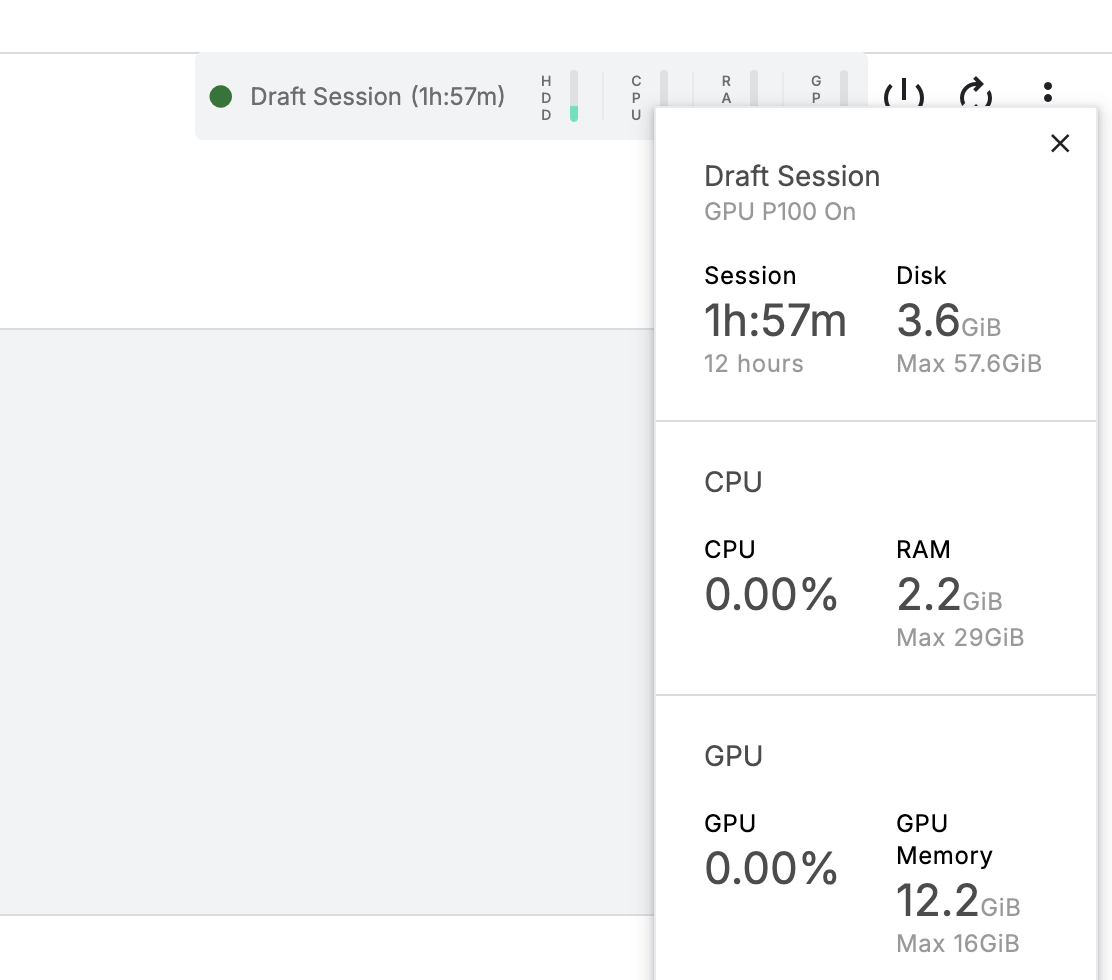
\includegraphics[width=0.4\textwidth]{pics/bert_consuming.png}
    \caption{BERT training environment}
\end{figure}

\subsection{Input data and processing}
This experiment based on BERT and IMDb dataset (like previous experiments). The original "stanfordnlp/imdb" dataset includes training and testing sets, so, we will use the pre-split sets to train and test this time. But we need to tokenize every sample for fine tuning the BERT model configured for classification task.

Compare to the generative LLMs (large language models), BERT needs structured data for its tasks.
The preprocessing steps include tokenizing the textural samples, the "BertTokenizer" from the transforms library, specifically the "google-bert/bert-base-uncased", is used to tokenize the reviews. The preprocessing follows the next steps:

\begin{enumerate}
    \item Tokenization: Converts raw content into tokens compatible with BERT.
    \item Truncation and Padding: Ensures all textual inputs are filled to a maximum length of 512 (in this experiment setting) tokens and padded to maintain uniform input size.
    \item Batched Processing: The training and testing sets are tokenized in batches to improve efficiency.
\end{enumerate}

\begin{figure}[ht]
    \centering
    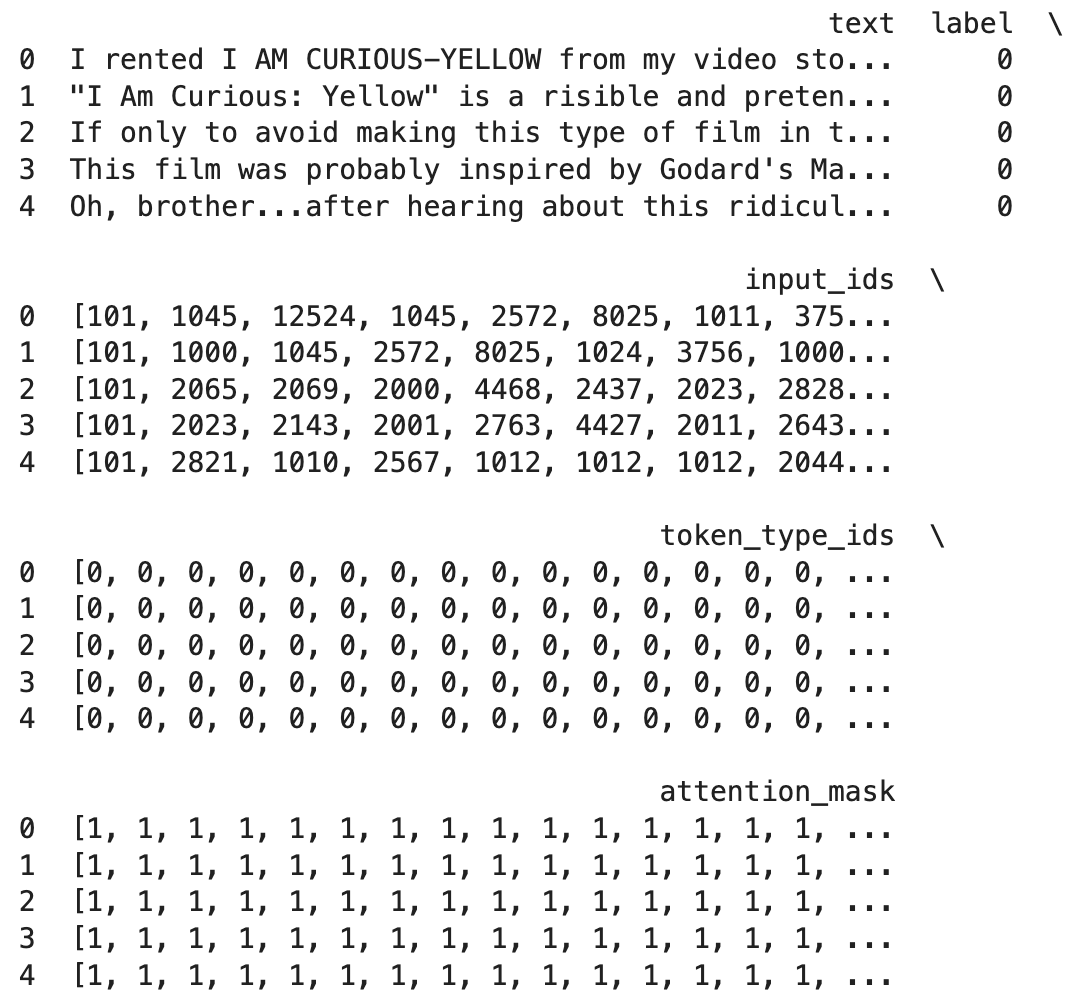
\includegraphics[width=0.6\textwidth]{pics/bert_data_treate.png}
    \caption{The structured data for BERT}
\end{figure}

\subsubsection*{Reasons for Tokenization}

\begin{itemize}
    \item Model Compatibility: BERT models require formatted inputs as the numerical token IDs instead of raw text. This process converts words into the IDs based on the pre-trained vocabulary dictionary.
    \item Fixed Length: BERT expects inputs with fixed length. 
    \item Efficient Processing: The batch processing is critical for efficient training on large datasets like IMDb.
    \item Special Tokens: BERT requires specific tokens (e.g., [CLS], [SEP]) to indicate the start and end of sequences, this step is done by tokenization automatically.
    \item Attention Masking: Tokenization generates attention masks to differentiate meaningful tokens from whole inputs to improve model efficiency by ignoring padded tokens.
\end{itemize}

\subsubsection*{Fields in Tokenized Data}

The "preprocess\_function" generates the dataset with the following fields for each sample:

\textbf{"input\_ids"}: A list of integers for representing the tokenized words of the review, mapped to the BERT vocabulary. Each ID in this list corresponds to a specific token. For example, the word "movie" might be mapped to a specific ID like 3185. This field is the primary input to the BERT model for processing the text.

\textbf{"token\_type\_ids"}: A list of binary integers (0 or 1) indicates the tokens belong to the first sequence (the review text) or a second sequence (e.g., a question in question-answering tasks). For this tasks with single sequence, such as sentiment classification, all values are typically 0. This field is working for compatibility with tasks involving multiple sequences.

\textbf{"attention\_mask"}: A list of binary integers indicates which tokens should be processed by the model (1 for real tokens, 0 for padding tokens). This list ensures the model ignores padding tokens added to reach the fixed length, and improves computational efficiency.

\textbf{"labels"}: The original label, 0 means negative and 1 means positive, is retained for training and evaluation. This field is also used to compute the loss during training.

% training and optimize
\subsection{Training(fine tuning) BERT model}
The used model is "BertForSequenceClassification", which from the transformers library and is initialized with the "google-bert/bert-base-uncased". This model is configured for binary classification by setting 'num\_labels' as 2. Training is conducted using the "Trainer" API from the transformers library with the following configuration:

\begin{itemize}
    \item Output Directory: Setting it as current dictionary for saving model, images or logs.
    \item Evaluation Strategy: Setting it off for improving training performance with limited resource.
    \item Learning Rate: Setting it as '2e-5', it is a standard choice for fine-tuning BERT models.
    \item Batch Sizes: Setting it as 32 for training and 64 for evaluation to lower time consuming.
    \item Epochs: Setting it as 3 to balance model's convergence and computational efficiency.
    \item Weight Decay: Setting it as 0.01 to prevent overfitting.
    \item Logging: Setting it as closed for much better performance.
\end{itemize}

\subsection{Optimization of Fine tuning}
This training experiences around 2 hours, which is much time consuming compared to the previous methods. This time consuming is the optimized results. For this method, the optimize is focusing on to run faster to ensure the experiment can be finished. So, we canceled the in-processing evaluation and logging which causes much slower training. We just use 3 epochs that normally used to train the model to prevent overfitting. In the future optimization, to use the larger BERT model like "" is the choice for better performance. 

\subsection{The Evaluation of BERT}

Although the evaluation strategy was set to "no" during training, after training, we can get "eval\_loss" as 0.2147 by invoking "trainer.evaluate" under training all samples. This value is lowering belong the number of samples increasing. The test dataset "tokenized\_test" is prepared for next post-training evaluation. The model is evaluated by Confusion Matrix, Classification Report and ROC Curve by importing "sklearn.metrics".

\begin{figure}[ht]
    \centering
    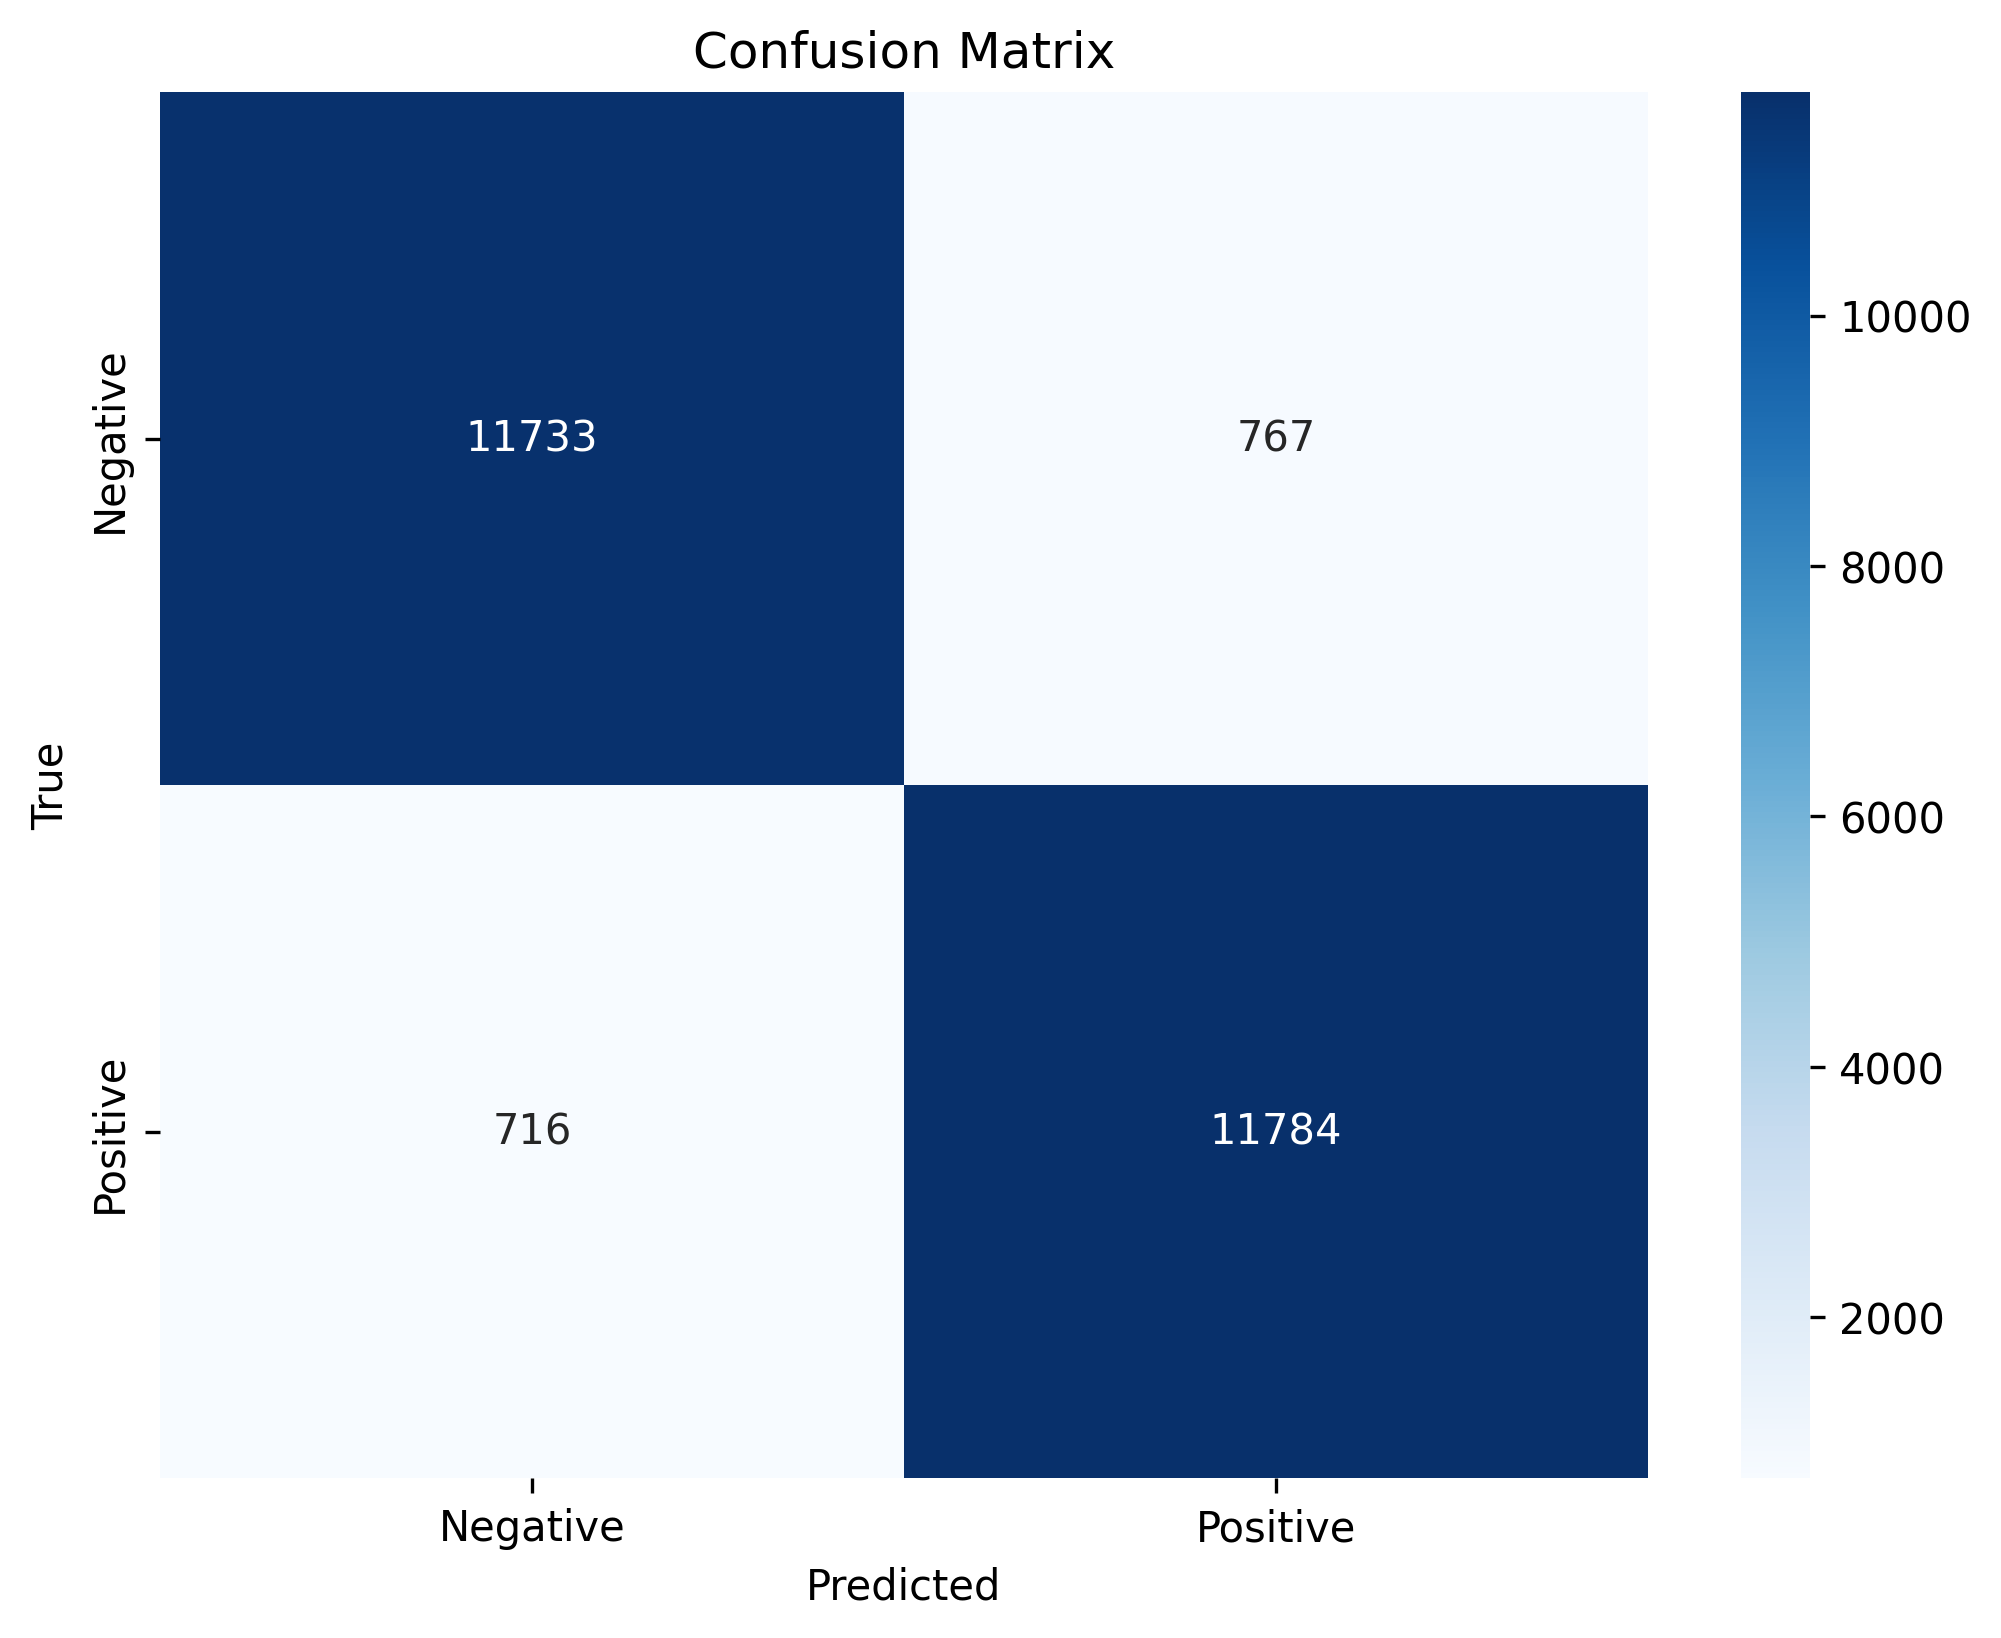
\includegraphics[width=0.4\textwidth]{pics/bert_matrix.png}
    \caption{Confusion Matrix of BERT}
\end{figure}

It is clear that the true positive and true negative is significantly higher than the false negative and false positive, which means that the performance of BERT in this task is much near the 100\%. Depend on the Classification Report of BERT, this experiment also demonstrate the clear trend. The total accuracy is 94\%, and the positive and negative subsets accuracy is also the same values due to the balanced dataset. The precision, f1 score and recall are also reached the perfect range of value.

The Receiver Operating Characteristic (ROC) curve for the BERT model illustrates its better performance in classifying task for positive and negative reviews, the curve demonstrates strong discriminative ability. The curve is expected to close the top-left corner, which reflects high True Positive Rate (TPR), and it gives the low evaluation loss of 0.2147 from "trainer.evaluate" method. 

\begin{figure}[ht]
    \centering
    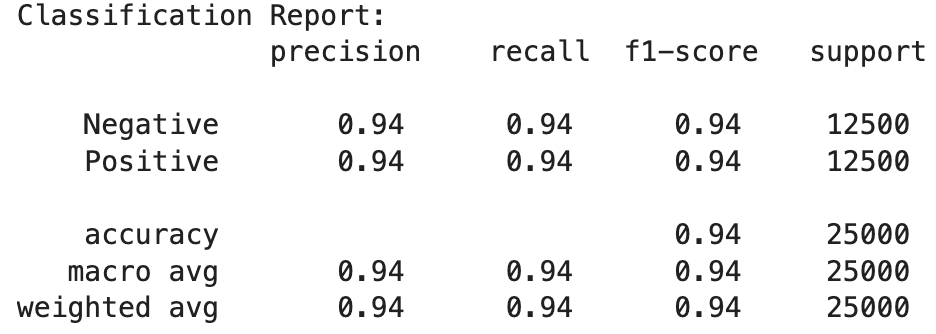
\includegraphics[width=0.5\textwidth]{pics/bert_eval_report.png}
    \caption{Classification Report of BERT}
\end{figure}

\begin{figure}[ht]
    \centering
    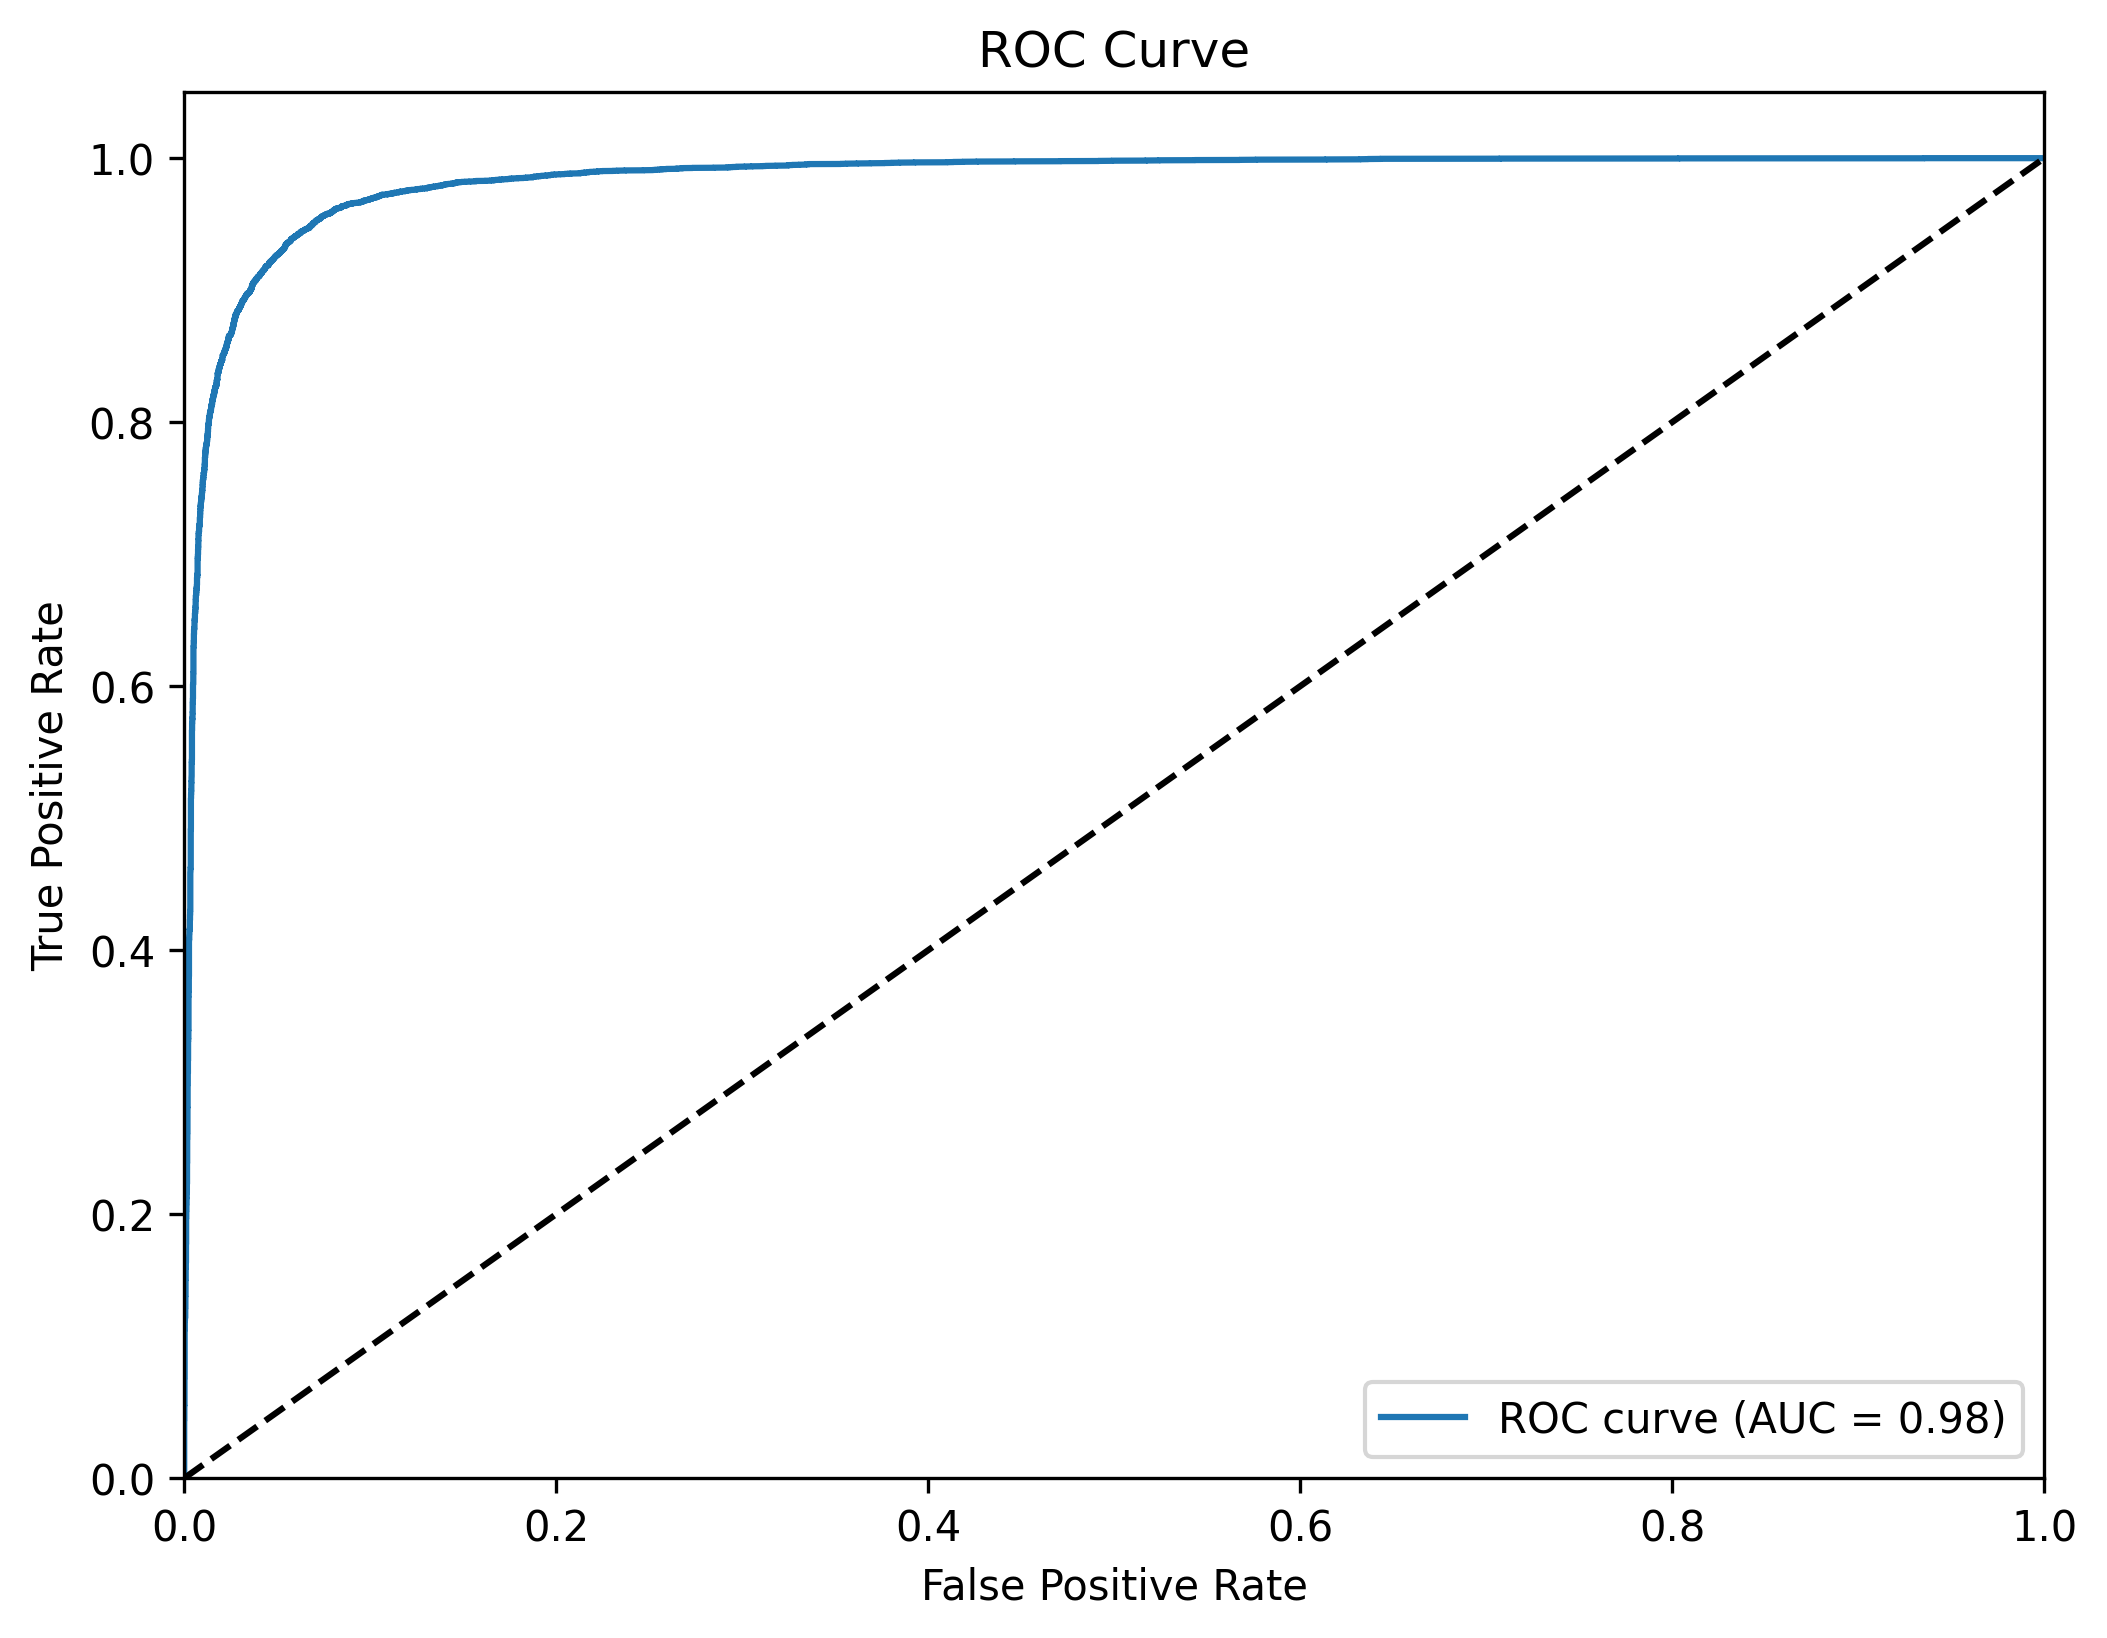
\includegraphics[width=0.5\textwidth]{pics/bert_roc_curve.png}
    \caption{ROC Curve of BERT}
\end{figure}

\subsection{Conclusion}
The experiment of this part demonstrates the successful application of the BERT model for sentiment classification on the IMDb dataset. The steady decrease in training loss over 2,346 steps indicates that the model effectively learned to classify movie reviews by positive or negative. The use of standard preprocessing techniques, such as tokenization with truncation and padding, ensure compatibility with BERT's input requirements. The training configuration, leveraging the Trainer API and GPU acceleration, was efficient and robust.